\chapter{Stato dell'arte}
\label{cha:statoArte}

\section{Reverse Proxy}
\begin{figure}[h!]
  \centering
  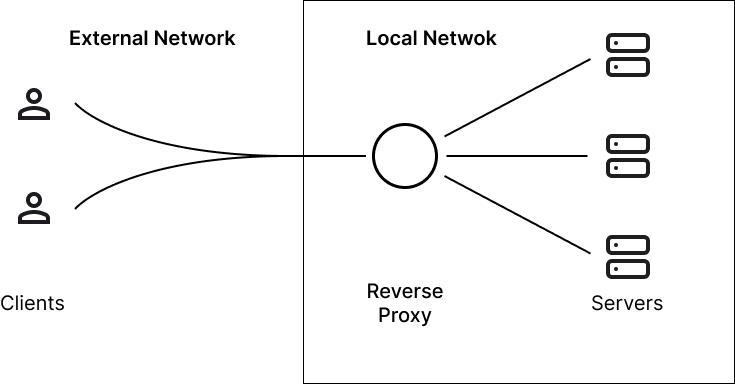
\includegraphics[width=.6\textwidth]{images/schema.png}
\end{figure}

\subsection{Cos'é}
Un reverse proxy é un dispositivo utilizzato nelle comunicazioni tra client e server. Questo dispositivo si interpone nelle comunicazioni nel lato dei server. Quindi viene utilizzato nella rete locale dove sono presenti i server e diventa l'unico nodo di accesso verso la rete globale. Ogni server quindi non sará direttamente collegato al client che effettua la richiesta, ma é collegato al reverse proxy che successivamente inoltrerá le richieste ai relativi servere e le risposte ai relativi client. Si fa ció cosí si dimiuisce il carico di lavoro ai server perché non devono effettuare i controlli di sicurezza, che vengono invece effettuati direttamente dal reverse proxy. Inoltre, visto che tutte le comunicazioni passano per quel nodo, si puó avere una visione piú generale di tutte le comunicazioni entranti e rilevare piú facilmente comportamenti anomali.
\subsubsection{Differenza con il forward proxy}
Il forward proxy é un dispositivo che funziana praticamente allo stesso modo peró si trova nelle rete locale dei client. Quindi se si hanno piú client ma si vuole avere solo un nodo di uscita verso la rete globale, si puó utilizzare un forward proxy.

\subsection{Esempio comunicazione}
\subsubsection{Elementi}
Client: C\\ Reverse Proxy: R\\ Server1: S1; Server2: S2
\subsubsection{Configurazione Reverse Proxy}
\paragraph{Dominio} Come esempio consideriamo il dominio \textit{example.com}. Quindi il reverse proxy risponderá alle richieste fatte a \textit{*.example.com}.
\paragraph{Routing} Definiamo in base al subdomain quale server deve essere indirizzato
\begin{enumerate}
  \item primo.example.com - server1 (172.17.0.1)
  \item secondo.example.com - server2 (172.17.0.2)
\end{enumerate}
\subsubsection{Comunicazione}
\begin{enumerate}
  \item
  \begin{verbatim}
    GET /index.html HTTP/1.1
    Host: primo.example.com
  \end{verbatim}
    C manda una richiesta tramite il dominio \textit{primo.example.com}
  \item
    \begin{verbatim}
    GET /index.html HTTP/1.1
    Host: 172.17.0.1
    \end{verbatim}
    R riceve la richiesta, vede che il dominio indicato ha \textit{primo} come sottodominio. Controlla nella configurazione e vede che \textit{primo.example.com} é collegato a S1. Crea quindi una richiesta uguale a quella ricevuta, cambiando il destinatario e indicando l'indirizzo ip di S1.
  \item R riceve la risposta alla richiesta da S1.
  \item R invia la risposta ricevuta a C.
\end{enumerate}


\subsection{Perché viene utilizzato}
L'utilizzo di una struttura che si pone in mezzo alle comunicazioni garantisce molti vantaggi visto che ha accesso a tutte le comunicazioni entranti. Il reverse proxy puó quindi analizzare le connessioni ed effettuare delle operazioni con queste ultime come ad esempio controlli per motivi di sicurezza, chaching e load balancing. Inoltre in questo modo si puó accedere a piú servizi tramite lo stesso nodo di ingresso.

\subsection{Funzionalitá}
Analizziamo adesso le funzionalitá che un reverse proxy puó offrire.

\subsubsection{Sicurezza}
Sicuramente le funzionalitá piú importanti sono quelle relative alla sicurezza. Un reverse proxy infatti ne implementa molte evitando la necessitá di implementare sistemi di sicurezza per ogni servizio che andiamo ad inserire nella rete locale.
\begin{enumerate}
  \item \textbf{TLS}: Le comunicazioni entranti ed uscenti dal reverse proxy possono essere criptate tramite il protocollo TLS, anche se un server non lo implementa. Quindi si possono effettuare le comunicazioni da server a reverse proxy in chiaro, e poi lasciare che diventi sicura solo dopo il reverse proxy.
  \item \textbf{controllo attacchi DoS/DDoS}: Controllando tutte le comunicazioni e i relativi ip sorgente, si possono applicare filtri e controlli per evitare un eccesso di richieste in entrata che possono rallentare le funzionalitá dei server. In questo modo se si rileva un'anomalia di richeste ad un server che fa presumere ad un attacco DoS, si possono bloccare direttamente le richieste ancora prima che arrivino al server.
  \item \textbf{supporto protocolli piú recenti}: Il reverse proxy puó supportare protocolli piú recenti rispetto ai server cosí la connessione interna tra servere e reverse proxy puó essere effettuata nel protocollo piú recente supportata dal server, ma poi quella all'esterno puó essere elevata ad un protocollo piú recente e quindi con maggiore sicurezza.

\end{enumerate}

\subsubsection{Prestazioni}
\begin{enumerate}
  \item \textbf{TLS}: Criptare la comunicazione nel nodo del reverse proxy e lasciando la comunicazione interna in chiaro allegerisce molto il carico di lavoro ai server.
  \item \textbf{Cache}: Implementando un sistema di caching, richieste ricorrenti alle stesse risorse possono essere soddisfatte direttamente dal reverse proxy, senza inoltrare la richiesta al server.
  \item \textbf{Compressione}: Comprimere le risposte cosí da occupare meno banda e non influire sulle prestazioni dei server in quanto il processo di compressione e decompressione delle richieste é effettuato dal reverse proxy.
\end{enumerate}

\subsubsection{Singolo IP}
Avendo solo un nodo collegato alla rete globale, si possono collegare molteplici servizi attraverso un solo indirizzo IP. Per fare ció si utilizzano i subdomain, cioé prefissi dell'URL base utilizzati per indirizzare risorse diverse. Con un reverse proxy si puó fare un'associazione subdomain -> server cosí da poterli indirizzare facilmente. La struttura dell'URL sará quindi \textit{http(s)://subdomain.example.com}.

\subsubsection{Load Balancer}
Se si hanno piú server (macchine) che rispondono alle stesse richieste, si possono indirizzare le richieste in modo che carico di lavoro sia distribuito equamente tra i vari server. In base all'algoritmo implementato il processo di load balancing puó essere fatto in modo accurato oppure piú grezzo. L'algoritmo scelto dipende molto dal caso d'uso.

\subsection{Criticitá}
\cite{risks}
\subsubsection{Aumento latenza}
Le richieste devono passare un nodo in piú nel loro viaggi o tra il client e il server. Questo implica un tempo di elaborazione del pacchetto da parte del nodo che non ci sarebbe stato altrimenti e quindi anche un aumento della durata totale della comunicazione.
\subsubsection{Singolo punto di rottura}
Avendo tutte le comunicazioni che passano per il reverse proxy, é immediato che questo dispositivo diventa un elemento molto critico. Avere un problema di funzionalitá a questo nodo compromette le comunicazioni dirette a tutti i server. Cosa che non succederebbe se ogni server avesse un accesso alla rete globale indipendente.
\subsubsection{Possibili colli di bottiglia}
Il carico di lavoro sul reverse proxy puó diventare molto grande se si inseriscono molti servizi a monte. La potenza necessaria per non avere problemi di rallenatmenti deve essere valutata quindi molto bene altrimenti ne risentono tutti i servizi a monte anche se il server associato a quel servizio non sta avendo un grande carico di lavoro.
\subsubsection{Sicurezza}
Ovviamente il reverse proxy serve per aumentare il livello di sicurezza ma sua volta, essendo un software, puó essere soggietto a falle di sicurezza. Bisogna quindi assicurarisi che la configurazione del dispositivo sia fatta in modo da non lasciare porte aperte a possibili attacchi e verificare sempre gli aggiornamenti.



\section{SSL/TLS}
\cite{tls}SSL (Secure Socket Layer) e TLS (Transport Layer Security) sono protocolli finalizzati a garantire privacy e sicurezza nelle comunicazioni web. Per fare ció utilizzano degli algoritmi per criptare le comunicazioni e fare in modo che solo chi é in possesso delle chiavi puó vedere il contenuto originale del messaggio. SSL é il protocollo vecchio nato nel 1995 e attualmente non piú utilizzato. Gli algoritmi utilizzati nel protocollo SSL sono attualmente obsoleti e troppo deboli rispetto alla capacitá computazionale delle macchine odierne. Una comunicazione puó essere quindi decriptata con relativa facilitá, facendo cadere le garanzie di privacy e sicurezza indicate precedentemente. TLS invece é il protocollo attualmente utilizzato, adesso arrivato alla versione 1.3. Questo é il protocollo uttualmente utilizzato e impiega algoritmi che attulamente sono ancora considerati sicuri in quanto estremamente difficili da aggirare con la potenza di calcolo di cui si dispone ora.
\subsection{Funzionamento TLS}
\subsubsection{Handshake}
Quando viene instaurata la connessione i primi messaggi inviati dalle due parti servono per effettuare l'handshake. Durante questa fase si vanno a decidere protocolli utilizzati, chiavi, nonce.
\begin{enumerate}
  \item \textbf{fase 1}: Nella prima fase si negoziano la versione di TLS da utilizzare i nonce e gli algoritmi da utilizzare per criptare i messaggi. I \textbf{nonce} sono numeri che identificano la sequenza dei messaggi inviati. Sia il server che il client hanno il proprio nonce, che verrá allegato al messaggio per identificare la comunicazione. Questo valore é importante perché se un soggetto malevolo volesse mandare un messaggio a una delle due parti dovrebbe sapere il valore del nonce, altrimenti il messaggio viene scartato immediatamente perché non appartenente ad una sessione valida.
  \item \textbf{fase 2}: Il server invia al client la chiave pubblica per verificare il certificato e la sua parte di parametri in caso venga utilizzato DH (Diffie-Hellman) come protocollo di condivisione della chiave.
  \item \textbf{fase 3}: Il client tramite la chiave pubblica del certificato verifica che il server é il vero possessore del certificato e invia al server is suoi parametri in caso di DH, oppure la chiave criptata con la chiave pubblica del server in caso di RSA.
\end{enumerate}
\subsubsection{Record}
I messaggi dopo quelli di handshake verranno poi criptati e verificato che non siano stati modificati.
\begin{enumerate}
\item \textbf{confidenzialitá}: il contenuto del messaggio deve essere visibile solamente alle 2 parti, se non si ha possesso delle chiavi non é possibile leggere il contenuto in chiaro.
\item \textbf{integritá}: se il messaggio é stato modificato nel mezzo della comunicazione, questo deve essere identificabile. Per effettuare ció si calcola il valore hash del messaggio e si cripta tramite una chiave negoziata. Il ricevente calcolerá poi il valore hash del messaggio ricevuto e se i 2 valori combaciano vuol dire che il messaggio non é stato modificato.
\end{enumerate}

\section{Certificati}
\cite{certificates}
I certificati servono per abilitare l'utilizzo di HTTPS, cioė la versione criptata del protocollo HTTP. I certificati sono coppie di chiavi (privata e pubblica) e altre informazioni relative al server che possiede il certificato. I certificati sono fondamentali nella comunicazioni per verificare che il server con cui si sta comunicando sia l'effettivo possessore del dominio a cui stiamo mandando le richieste.
\subsection{Informazioni contenute nel certificato}
\begin{enumerate}
  \item dominio e sottodomini
  \item chiave pubblica
  \item chiave privata (questa non viene condivisa con il client)
  \item ente che ha emesso il certificato
  \item informazioni sul possessore del certificato
  \item informazioni sulla chiave pubblica
  \item data di scadenza
  \item data di emissione

\end{enumerate}
\subsection{Chain of Trust}
Per fare in modo che un utente si possa fidare del certificato appartenente al server si utilizza un sistema chiamato Chain of Trust. Esistono degli enti che rilasciano chiavi a cui viene data fiducia a prescindere (root of trust). Questi enti rilasciano a degli altri enti di rilascio chiavi delle chiavi. Quando gli enti del secondo livello rilasciano le chiavi, nella loro chiave viene segnato che é stata rilasciata da uno degli enti di primo livello. Quindi se un server si fa rilasciare una chiave da un ente di secondo livello, l'utente nella chiave vedrá che é stato rilasciato da un determinato ente di secondo livello che a sua volta ha una chiave rilasciata da un ente di primo livello. L'utente andrá quindi a vedere se questo ente di primo livello é presente nella lista degli enti a cui viene data fiducia e se sí il collegamento puó continuare senza problemi.

\subsection{Come verificare un certificato}
Per assicurarsi che il server sia il vero possessore della chiave privata del certificato si fá criptare un messaggio dal server con la sua chiave privata e poi il cliente lo decripta con la chiave pubblica. Quindi l'unico modo per costruire un messaggio che poi decriptato con la chiave pubblica abbia un senso é avendo la chiave privata. Il server quindi calcola un hash value di alcune informazione relative al certificato e che vengono condivise con il client e poi lo cripta con la chiave pubblica. Invia il valore al client che lo decripterá con la chiave pubblica. Il client calcola a sua volta lo stesso hash value e poi lo compara con quello ricevuto dal server. Se i 2 combaciano vuol dire che il server possiede la chiave privata giusta e quindi il client si puó fidare.

\section{Container}
\subsection{Cosa sono}
\cite{container}I container sono software eseguibili che contengono tutte le dipendenze per essere eseguiti come librerie, binari e file di configurazione. Indipendentemente dal sistema "host", cioé il sistema su cui viene eseguito il container, quest'ultimo funzionerá sempre allo stesso modo. Per uno sviluppatore questo é molto importante perché altrimenti dovrebbe creare delle versioni diverse dello stesso software per adattarle a ogni tipo di sistema operativo.
\subsection{Differenze dalle macchine virtuali}
\begin{enumerate}
  \item \textbf{kernel}: I container si appoggiano sul kernel del sistema operativo ospitante, mentre le macchine virtuali sono un sistema operativo che gira sopra il sistema operativo ospitante, con anche l'hardware che viene simulato. Questa differenza rende i container molto piú leggeri sia come utilizzo di risorse che come dimensione effettiva del software.
  \item \textbf{isolamento}: I container isolano il software a livello di processo, mentre le chiamate kernel fanno affidamento al sistema operativo ospitante. Le macchine virtuali invece non condividono niente col sistema operativo ospitante in quanto un nuovo sistema operativo é emulato per intero. Questo maggiore isolamento peró non é necessario nella maggiore parte dei casi, almeno che non vengano utilizzate queste tecnologie per offrire dei servizi dove gli utenti posson eseguire del codice all'interno dell'ambiente virtualizzato. In questo caso é meglio avere l'ambiente completamente isolato.
\end{enumerate}

\subsection{Docker}
\cite{docker}Docker é attulamente il software maggiormente utilizzato per la creazione, gestione ed esecuzione dei container. La sua popolaritá é dovuta principalmente alla semplicitá di utilizzo e alla gestione dei container. Infatti per creare un container bisogna creare un file dove vengono scritte le direttive per compilare il progetto e i comandi da eseguire quando il container viene eseguito. La gestione risulta inoltre comoda in quanto c'é un sistema di versionamento dei container, in stile git, che rende la gestione delle versioni comoda.

\subsection{Kubernetes}
Kubernetes é un ulteriore software che rende la scalabilitá dei container piú facile ed efficiente. Con kubernetes infatti si possono eseguire dei servizi utilizzando le risorse di diverse macchine. Quindi se si hanno molteplici macchine e un servizio molto difficile da eseguire, tramite kubernetes si possono dividere le operazioni su queste macchine.
